\documentclass[10pt, a4paper]{article} % 设置字体大小和纸张类型
\usepackage{ctex}
\usepackage{caption} % 插图和表格的标题格式
\usepackage{amsmath, amsfonts, amssymb} % 数学公式支持
\usepackage{graphicx} % 插入图片
\usepackage{hyperref} % 超链接支持
\usepackage{geometry}
\usepackage{titlesec}
\usepackage{fmtcount} % 用于数字到中文的转换
\usepackage{enumitem} % 加载 enumitem 宏包
\usepackage{amsmath} % 加载 amsmath 宏包以增强数学公式排版
\usepackage{booktabs} % 支持更专业的表格线条
\usepackage{multirow} % 支持多行单元格
\usepackage{makecell}
\geometry{a4paper, margin=1.5cm} % 设置页边距

\renewcommand{\thesection}{\chinese{section}、}
\renewcommand{\thesubsection}{\arabic{subsection}.}


\begin{document}

\begin{titlepage}
    \newgeometry{left=0cm, right=0cm, top=0cm, bottom=0cm}
    \centering
    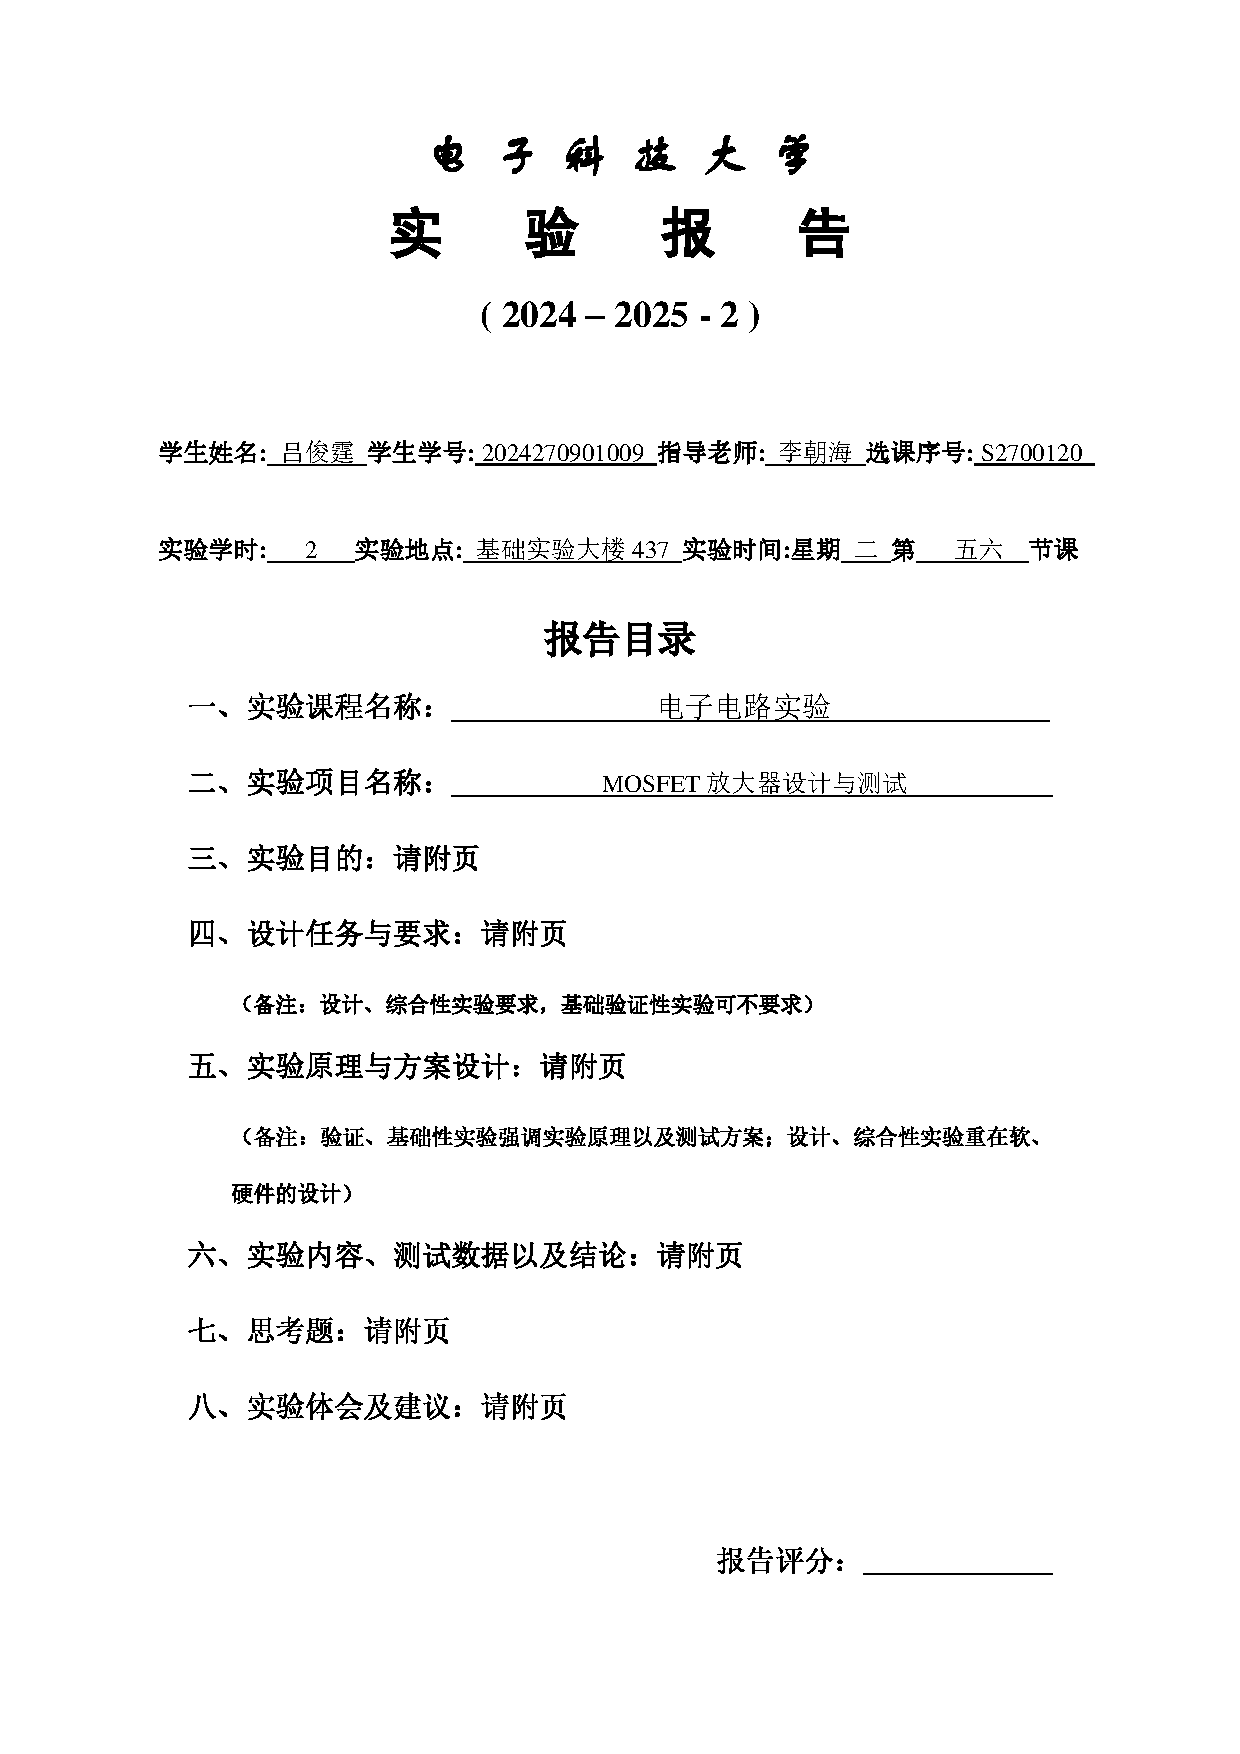
\includegraphics[page=1, width=0.9\textwidth, keepaspectratio]{image/实验报告撰写封面.pdf}
    \restoregeometry
\end{titlepage}

\setcounter{section}{2}

\section{实验目的}

\begin{enumerate}[leftmargin=50pt,label=(\arabic*)] % 设置序号格式为(1)
    \item 理解 MOSFET 放大电路的组成原则、组成方式特点和电路特点; 
    \item 掌握 MOSFET 放大电路静态工作点的测试方法和调试原理; 
    \item 掌握 MOSFET 放大电路增益(放大倍数)的测试方法;
    \item 掌握 MOSFET 放大电路输入电阻、输出电阻和通频带的测试方法;
    \item 掌握直流稳压电源、数字万用表、函数发生器、晶体管毫伏表和示波器的使用方法。
\end{enumerate}

\section{设计任务与要求}

暂不需要。

\section{实验原理与方案设计}
\subsection{实验原理}
场效应管是一种电压控制型的半导体器件。按其结构和工作原理不同,可分为结型场效 应管和绝缘栅型场效应管。它不仅像双极型晶体管一样具有体积小、重量轻、耗电少、寿命长等优点;而且与 BJT 相比, 它的输入阻抗很高, 可达10$G\omega$以上。热稳定性好, 抗辐射 能力强。它的最大优点是占用硅片面积小,制作工艺简单,成本低,很容易在硅片上大规模集成,因此在大规模集成电路中占有极其重要的地位。

(1) 绝缘栅型场效应晶体管(MOSFET)的结构和特性
\vspace{0.5cm}


\begin{figure}[ht]
    \centering
    \begin{minipage}[ht]{0.46\textwidth}
        \centering
        绝缘栅型效应管(MOSFET)简称 MOS 管, 由金属、氧化物、半导体材料制成,因其栅极与其它电极完全绝缘而得名。绝缘栅型效应管按照导电沟道有 N沟道和 P沟道之分外, 还可以根据工作方式的不同分为增强型和耗尽型。
        
    \end{minipage}
    \hfill
    \begin{minipage}[ht]{0.46\textwidth}
        \centering
        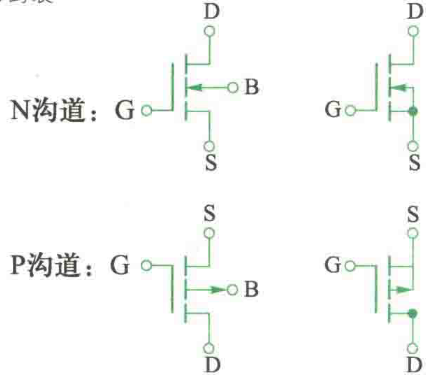
\includegraphics[width=\linewidth]{image/1.png}
        \caption{图为增强型MOSFET电路图符号}
        \label{fig:side:a}
    \end{minipage}
\end{figure}

NMOS管I-V特性
\vspace{0.5cm}
图2所定义的电压栅源电压\(V_{GS}\)和漏源电压\(V_{DS}\)之间的关系, 可以用转移特性曲线来描述, 如图3所示。输出电压\(V_{DS}\)与漏极电流\(I_{D}\)之间的关系, 可以用输出特性曲线来描述, 如图4所示。

I. 截止区。当\(V_{GS} < V_{TH}\)时, 管子处于截止区, \(I_{D} = 0\);

II. 可变电阻区。当\(V_{GS} > V_{TH}\)时, 沟道形成, 如果此时\(v_{DS} > 0\), 沟道内的电子运动将形成漏极电流\(I_{D}\)。当\(v_{DS} < v_{GS} - V_T\)时, \(v_{DS}\)较小, $i_{D}$随$v_{DS}$基本作线性变化, 可视为一定斜率的直线, 形成沟道导通电阻。当$v_{GS}$变化时, 沟道导通电阻也随之变化, 从而形成可变电阻区。

III. 饱和区。当\(v_{DS} > v_{GS} - V_T\)时, 沟道内的电子运动将形成漏极电流\(I_{D}\)基本不随电压变化。此时, 沟道内的电子受到漏极电压的影响, 电子的速度减小, 电子的迁移率减小, 沟道内的电子浓度减小, 沟道导通电阻增大, 沟道导通电阻不再是线性变化, 而是随着漏极电压的增大而减小, 从而形成饱和区。

\begin{figure}[ht]
    \centering
    \begin{minipage}[ht]{0.3\textwidth}
        \centering
        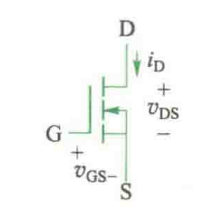
\includegraphics[width=\linewidth]{image/2.png}
        \caption{电压电流定义}
        \label{fig:side:b}
    \end{minipage}
    \hfill
    \begin{minipage}[ht]{0.3\textwidth}
        \centering
        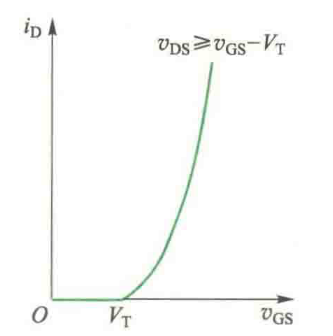
\includegraphics[width=\linewidth]{image/3.png}
        \caption{转移特性曲线}
        \label{fig:side:c}
    \end{minipage}
    \hfill
    \begin{minipage}[ht]{0.3\textwidth}
        \centering
        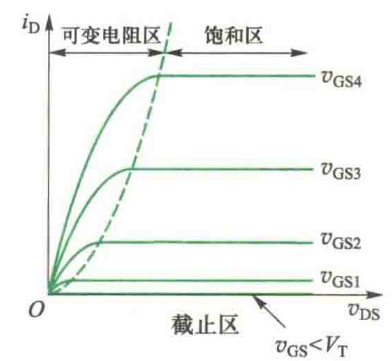
\includegraphics[width=\linewidth]{image/4.png}
        \caption{输出特性曲线}
        \label{fig:side:d}
    \end{minipage}
    
\end{figure}

\newpage

当NMOS管处于不同工作区域时, 其I-V特性如下:

$$
i_{\mathrm{D}} = 
\begin{cases} 
0, & \text{截止区} \\
K \left[ (v_{\mathrm{GS}} - V_{\mathrm{T}}) v_{\mathrm{DS}} - \frac{1}{2} v_{\mathrm{DS}}^2 \right], & \text{可变电阻区} \\
\frac{1}{2} K (v_{\mathrm{GS}} - V_{\mathrm{T}})^2, & \text{饱和区(忽略沟道长度调制效应)}
\end{cases}
$$ 
其中K为NMOS管工艺相关的跨导参数, 单位为A/V$^2$。


(2) 共源极 MOSFET 放大电路分析
\vspace{0.5cm}

图5所示为阻容耦合共源极放大电路。为使MOS管工作在恒流区, 通过$R_{g1}$和$R_{g2}$对电源$V_{DD}$分压来设置偏压$V_{GQ}$, 所以称此电路为分压式偏置电路。$V_{GS}$应大于开启电压$V_{T}$; 在输出回路所加的漏极电源$V_{DD}$, 一方面时漏源电压大于夹断电压, 以保证管子工作在恒流区, 另一方面作为电路的能源。$R_d$的作用时将漏极电流$i_D$的变化转换成电压$v_{DS}$的变化, 从而实现电压放大。

\begin{figure}[ht]
    \centering
    \begin{minipage}[ht]{0.6\textwidth}
        \centering
        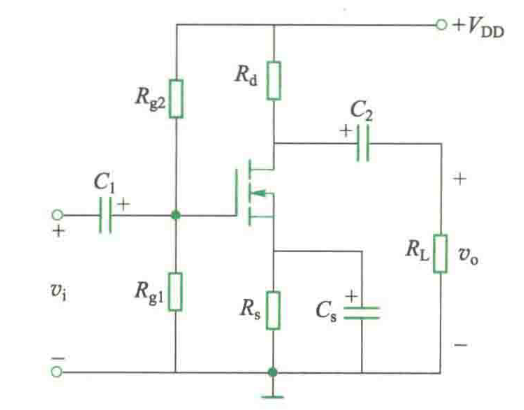
\includegraphics[width=\linewidth]{image/5.png}
        \caption{电路原理图}
        \label{fig:side:e}
    \end{minipage}
    \hfill
    \begin{minipage}[ht]{0.35\textwidth}
        \centering
        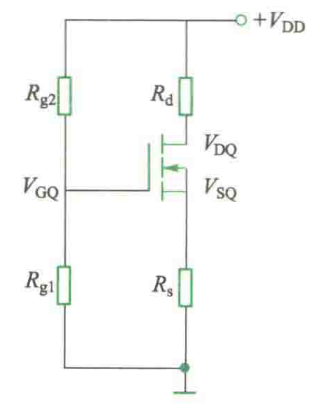
\includegraphics[width=\linewidth]{image/6.png}
        \caption{分压偏置电路}
        \label{fig:side:f}
    \end{minipage}
\end{figure}

1.直流分析

据放大电路得到图6所示的分压偏置电路, 由于MOS管的栅极电流极小, 可忽略不计, 故栅极电位可用分压公式得出
$$
V_{GQ} = V_{DD} \cdot \frac{R_{g2}}{R_{g1} + R_{g2}}
$$
而源极电压
$$
V_{SQ} = I_{DQ} \cdot R_{S}
$$
因此: 
$$
V_{GSQ} = V_{GQ} - V_{SQ} = \frac{R_{g2}}{R_{g1} + R_{g2}} \cdot V_{DD} - I_{DQ} \cdot R_{S}
$$
假设MOSFET工作于饱和区, 在葫芦沟道长度调制效应的条件下, 有
$$
I_{DQ} = \frac{1}{2} K (V_{GSQ} - V_{T})^2
$$
选定MOSFET后, K和$V_{T}$是常数, 由上式可得出$I_{DQ}$, $V_{GSQ}$。可得出漏源工作点电压$V_{DSQ}$为
$$
V_{DSQ} = V_{DD} - I_{DQ} \cdot (R_{D}+R_{S})
$$
求解得到的$V_{GSQ}, I_{DQ}, V_{DSQ}$为MOSFET放大电路的静态工作点。

2.动态分析

把场效应晶体管用低频小信号模型替代得到图7所示的共源放大器的交流小信号等效电路(不考虑沟道调制效应)。场效应晶体管放大电路的动态分析时根据微变等效电路求电路的电压放大倍数$A_v$、输入电阻$R_i$、输出电阻$R_o$。
\begin{figure}[ht]
    \centering
    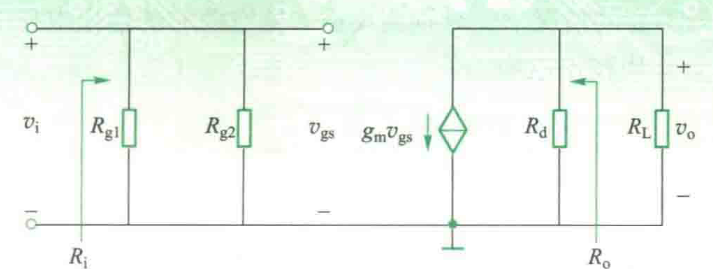
\includegraphics[width=0.7\linewidth]{image/7.png}
    \caption{交流小信号等效电路}
    \label{fig:side:g}
\end{figure}

I.电压放大倍数

根据电压放大倍数的定义计算可得
$$
A_v = \frac{v_o}{v_i} = -g_m \cdot (R_d || R_L)
$$
II.输入电阻
$$
R_i = R_{g1} || R_{g2} 
$$
III.输出电阻
$$
R_o = R_d
$$

(3) 场效应晶体管放大电路的测试方法
\vspace{0.5cm}

I.静态工作点的测试方法

测量放大器的静态工作点, 应在不加输入信号($v_i = 0$)的情况下进行。

场效应晶体管放大电路的静态工作点测量可选用量程合适的数字万用表(也可以使用示波器直流耦合方式测量), 分别测量场效应晶体管各电极对地的电位$V_{GQ}$、$V_{SQ}$和$V_{DQ}$。对漏极静态电流的测量, 为了避免断开漏极, 可使用间接测量的方法, 即先测量源极电阻$R_S$的两端电压, 再根据$V_{SQ} = I_{DQ} \cdot R_S$计算$I_{DQ}$。为了减小误差, 提高测量精度, 应选用内阻较高的直流电压表。

II.动态指标的测量

A.电压放大倍数的测量

电压放大倍数的测量, 可以通过输入一个幅度为$V_i$的正弦信号, 测量输出信号的幅度$V_o$, 由此计算电压放大倍数
$$
A_v = \frac{V_o}{V_i}
$$。
B.输入电阻的测量

当被测电路的输入电阻不太高时, 可以在信号源与放大器的输入端之间串接入一已知取样电阻R, (与$R_i$为同一数量级), 用交流电压表分别测出取样电阻R两端对地的电压$V_R$和$V_i$, 由此计算输入电阻
$$
R_i = \frac{V_i}{V_R-V_i} \cdot R
$$。

C.输出电阻的测量

在保证输入信号不变的情况下, 分别测出放大器空载时的输出电压$V_o$和接有负载时的输出电压$V_{oL}$, 由此计算输出电阻
$$
R_o = \frac{V_o - V_{oL}}{V_{oL}} \cdot R_L
$$。

D.幅频特性的测量

用点频法, 即保持输入信号大小不变, 改变输入信号的频率, 测量对应的输出电压值, 由此绘制幅频特性曲线。

\section{实验内容、测试数据以及结论}

用给定的NMOS管2N7000设计共源放大器。开启电压为$V_T$=1.5~2V, 跨导参数K=0.1A/V$^2$。已知$V_{DD}=12V$, 设计要求:$A_v > 20$、$R_o < 5K\omega$, 能不失真地放大峰峰值为30mV的正弦信号。

(1)静态工作点调整与测试

令$V_{DD} = +12V$, 用万用表测量$V_G$、$V_S$、$V_D$, 计算静态工作点$V_{GSQ}$、$I_{DQ}$、$V_{DSQ}$。

\begin{table}[ht]
    \centering
    \label{tab:a}
    \begin{tabular}{c|c|c|c|c|c}
        \toprule
        $V_{DD}(V)$&$V_{GQ}(V)$&$V_{SQ}(V)$&$V_{DQ}(V)$&$I_{DQ}(mA)$&$V_{DSQ}(V)$\\
        \midrule
        1.13&2.68&9.62&1.55&0.11&8.49\\ 
        \bottomrule
    \end{tabular}
\end{table}

(2)电压放大倍数的测量

用函数发生器输出一个正弦波信号作为放大器的输入信号, 设置信号频率f=1kHz, 幅度$V_i$=10mV, 测量输出信号的幅度$V_o$, 计算电压放大倍数$A_v$。

\begin{table}[ht]
    \centering
    \label{tab:b}
    \begin{tabular}{c|c|c|c|c}
        \toprule
        测试条件&工作状态&输出电压($V_o$)&放大倍数($A_v$)&输出波形\\
        \midrule
        \makecell{f=1kHz \\ $V_i$=10mV}&饱和&250mV&25&正弦波\\ 
        \bottomrule
    \end{tabular}
\end{table}

(3)输入电阻的测量

在放大器输入口串接一个取样电阻R, 用“两次电压法”测量该放大器地输入电阻$R_i$。
\begin{table}[ht]
    \centering
    \label{tab:c}
    \begin{tabular}{c|c|c|c}
        \toprule
        $V_s$&$V_i$&取样电阻R&$R_i$\\
        \midrule
        20mV&7.9mV&30K$\omega$&19.58K\\ 
        \bottomrule
    \end{tabular}
\end{table}

\newpage

(4)输出电阻的测量
在放大器输出口选择一个合适的负载电阻$R_L$, 运用“两次电压法”分别测量空载与接上负载时地输出电压值$V_{o}^{'}$和$V_o$。

\begin{table}[ht]
    \centering
    \label{tab:d}
    \begin{tabular}{c|c|c|c}
        \toprule
        $V_{o}^{'}$&$V_o$&负载电阻$R_L$&$R_o$\\
        \midrule
        480mV&250mV&2K$\omega$&1.84K\\ 
        \bottomrule
    \end{tabular}
\end{table}

(5)幅频特性的测量

用点频测试法测量放大器空载时地频率特性, 并求出带宽。

\begin{table}[ht]
    \centering
    \label{tab:e}
    \begin{tabular}{c|c|c|c|c|c|c|c|c}
        \toprule
        \multirow{2}{*}{频率值/Hz}&$\frac{f_L}{2}$&$f_L$&$\frac{f_0}{2}$&$f_0$&2$f_0$&$f_H$&2$f_H$&\multirow{2}{*}{带宽$\Delta f$}\\
        \cline{2-8}
        13&26&52&500&1K&2K&286K&572K\\
        \midrule 
        $V_o^{\prime}/V$&230mV&340mV&480mV&480mV&480mV&340mV&200mV&286K\\
        \bottomrule
    \end{tabular}
\end{table}

绘制图像如图

\begin{figure}[ht]
    \centering
    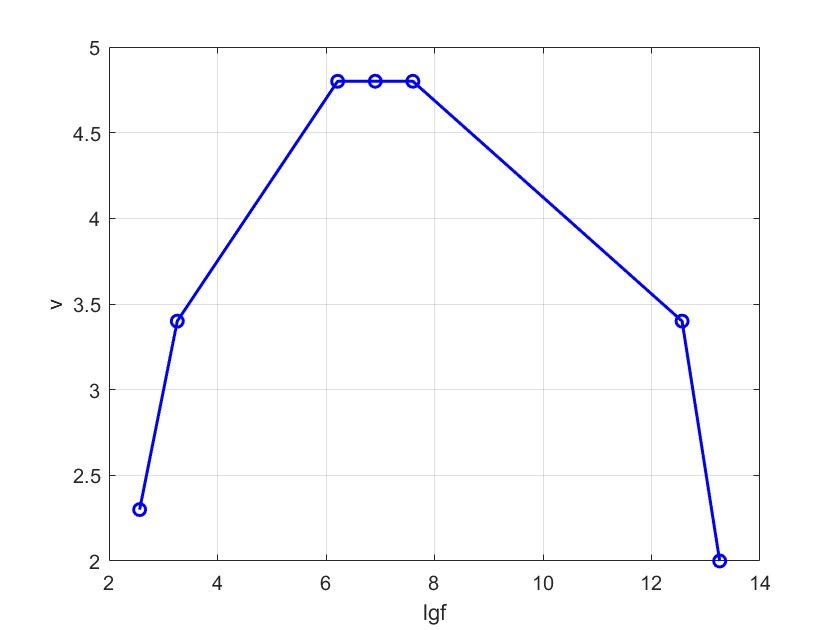
\includegraphics[width=0.7\linewidth]{image/1.jpg}
    \label{fig:side:h}
\end{figure}

\subsection{实验结论}

1.输入信号的频率大小会影响放大器的放大倍数, 且在一定范围内的频率可以使放大器的放大倍数稳定在一个较高的水平。

2 实验前应估算好输入电阻、输出电阻的大小, 电阻阻值的选择会影响放大器放大的效果。

\section{思考题}
\subsection{题面}
\begin{enumerate}[leftmargin=50pt,label=(\arabic*)] % 设置序号格式为(1)
    \item 场效应管放大电路和双极型管放大电路性能有何差别?
    \item 测量输入信号电压有效值、输出信号电压有效值时, 要采用交流毫伏表而不用数字万用表, 为什么?
    \item 测量场效应管放大电路输入电阻时可以采用其他的测量方法?
    \item 思考共漏极放大电路的分析与测量方法。
\end{enumerate}
\subsection{回答}

\begin{enumerate}[leftmargin=50pt,label=(\arabic*)] % 设置序号格式为(1)
    \item 场效应管放大电路的输入阻抗远高于双极型管放大电路。
    \item 数字万用表有一定的通频带, 只能测量较低频的信号, 超过这个范围会产生失真。毫伏表比数字万用表更高端, 很好地避免了失真问题。
    \item 可以采用电阻分压法、半压法等方法来进行测量。
    \item 共漏极放大电路的直流偏置电路与共源极放大电路完全相同,静态工作点的分析方法也和共源极放大电路相同。因此两者可以使用相似的办法进行分析与测量。
\end{enumerate}

\section{实验体会及建议}
\subsection{实验体会}
测量时应注意小心调试仪器, 尽量将读数稳定在误差允许范围内进行读数。
\subsection{建议}
注意仪器正负极的接入,防止反接造成仪器损坏。


\end{document}
